\documentclass[12pt]{article}
\usepackage[letterpaper, margin=1in]{geometry}
\usepackage{titlesec}
\usepackage{titling}
\usepackage{graphicx}
\usepackage{float}
\usepackage{url}
\usepackage{color}
\usepackage{siunitx}
\usepackage{natbib}
\usepackage{subcaption}
\usepackage{amsmath,amssymb,amsfonts}
\usepackage[colorlinks=true, urlcolor=blue, linkcolor=blue, citecolor=blue]{hyperref}


% Title formatting courtesy of Damein Koon
\pretitle{\LARGE\bfseries}
\posttitle{\par\vspace{2em}}
\preauthor{\large}
\postauthor{\par\vspace{1em}}
\predate{\large}
\postdate{\par\vspace{3em}}

% Corrected title hooks for vertical and horizontal centering
\renewcommand\maketitlehooka{\null\vfill\begin{center}}
\renewcommand\maketitlehookd{\end{center}\vfill\null}

\title{Machine Learning Stellar Classification}
\author{Krupa Pothiwala \\[0.5em]
May 2026}
\date{}

\begin{document}
\maketitle

\begin{abstract}
This project investigates whether unsupervised machine learning can rediscover known stellar populations in the NGC 2516 open cluster. It uses raw data from the Gaia DR3 catalog, without any prior information about the stars. PCA was applied first to 2,670 member stars filtered by parallax and proper motion, compressing the data into two principal components that captured $99.7\%$ of the total variance. These components mapped directly onto stellar brightness and distance, recovering the primary structure of the Hertzsprung-Russell diagram without any prior knowledge of stellar physics. UMAP and HDBSCAN were applied to the results of the PCA. However, they didn't add any new insights that were scientifically meaningful. Given that PCA alone produced clear, physically interpretable results with considerably less complexity, it was adopted as the final method.
\end{abstract}
\newpage

\section{Background Information}
The Hertzsprung-Russell (HR) diagram tells us what place a star occupies is in its life cycle. It is a very important tool in astronomy. It's like a map that shows us how stars change over time. If you look at the diagram, you'll see a big diagonal line running through the middle - that's called the Main Sequence (MS). This is where most stars spend their lives, and it's where our sun is right now. In the top right corner is the giants and supergiants, which are huge stars that have gone through main sequence. You can also see the "turn off" point which is where the main sequence stars star diverging into the supergiants or giants part of their life. In the bottom left corner there are white dwarfs which are stars that have gone through the giants and supergiant phase of their life. By looking at HR diagram astronomers can tell a lot of stars and stellar clusters.
\newline
\\There are certain terms that will be used throughout this project that are important to note:
\begin{itemize}
    \item mas - milliarcsecond, an angular measurement unit.
    \item G band - G filter on the telescope, measures white light around 330--1050 nano metres.
    \item parsec ($\varpi$) - unit of length used in astronomy. 3.26 light years $\approx$ 1 parsec.
    \item parallax - distance measurement (mas). Formula used for it is parsecs $=1000/\varpi$.
    \item proper motion (pm) - apparent angular motion of a star across the sky over time.
    \item apparent magnitude ($m$) - Brightness of a star as it appears to us. Depends on the band.
    \item absolute magnitude ($M$) - Brightness of an object if it were 10 parsecs away from Earth. Normalised magnitude. Depends on the band.
    \item Extinction ($A$) - how much light gets absorbed between us and the object due to dust and gas. Depends on the band. $A_G$ is the extinction speciafically in the G band.
    \item radial velocity - how much a star is moving towards or away from us (radially)
    \item ADQL - Astronomical Data Query Language. This isn't as important for the report but for the code there are certain words that I used because the Gaia databased required those trigger words \cite{adql}.
    \item RUWE - Renormalized Unit Weight Error. A Gaia quality metric for the astrometric fit. RUWE $\approx 1.0$ indicates a well-behaved single-star solution; RUWE $\geq 1.4$ suggests poor astrometry, often caused by unresolved binary companions \citep{pearce2022ruwe}.
    \item BP/RP bands - Blue Photometer and Red Photometer filters on Gaia. BP covers approximately 330--680 nm and RP covers approximately 640--1050 nm. Together with G band they form Gaia's three photometric bands.
    \item Color excess $E(\text{BP}-\text{RP})$ - The reddening correction applied to the color index. Dust scatters blue light more than red, making stars appear redder than they are. Subtracting this gives the intrinsic color $(BP-RP)_0$.
    \item Main sequence - The diagonal band on the HR diagram where stars spend most of their lives fusing hydrogen in their cores.
    \item Turn-off point - The location on the HR diagram where stars begin to leave the main sequence as they exhaust their core hydrogen. Its position indicates the age of the cluster.
    \item RA $\&$ Dec - Right ascension and declination are celestial coordinates similar to longitude and latitude for Earth. Declination is north or south from the celestial equator and right ascension measures east or west along the celestial equator in hours, minutes, and seconds.

\end{itemize}

\section{Data}
The stellar data was retrieved from the Gaia Data Release 3 (DR3) \cite{gaia_dr3} catalog using the \texttt{astroquery.gaia} \cite{astroquery_gaia} Python library, which provides access to the European Space Agency's Gaia archive \cite{gaia_archive}. A cone search was performed centered on NGC 2516 (RA $= 119.517^{\circ}$, Dec $= -60.752^{\circ}$) with a search radius of $1.0^{\circ}$. To pre-filter for likely cluster members, the query applied loose constraints on parallax ($1.5$--$3.5$ mas) and proper motion (pmRA $= -4.7 \pm 3.0$ mas/yr, pmDec $= 11.2 \pm 3.0$ mas/yr), consistent with published values for NGC 2516. Only stars with a parallax error below 0.5 mas and a valid G-band magnitude were included. The query was submitted as an asynchronous job with no row limit, returning photometric and astrometric columns including apparent magnitudes, color indices, proper motions, parallax, and extinction estimates.

\section{Cleaning}
After getting the raw data, a series of cleaning and engineering steps were taken to make sure that only reliable, usable stars were left. The first thing we did was get rid of any rows that didn't have core columns, like apparent magnitude, parallax, color index, and proper motion. These measurements are very important for all future analysis. Then, a standard Gaia quality cut was made using the RUWE metric (Renormalised Unit Weight Error) \cite{pearce2022ruwe}, which tells us how well the astrometric fit is for a given source. Any star with an RUWE $\geqslant 1.4$ was removed, which is the standard way to mark unreliable astrometric solutions. From the information provided by the database, two new columns were derived: absolute magnitude ($M_G$), calculated from apparent magnitude, parallax-based distance, and the G-band extinction using the distance modulus formula:
\begin{equation}
    M_G = m_G - 5\log_{10}(d) + 5 - A_G
\end{equation}
And the corrected color index:
\begin{equation}
    (BP - RP)_0 = (BP - RP) - E(BP-RP)
\end{equation}
The corrected color index subtracts the reddening estimate ($E(BP-RP)$) to remove the effect of interstellar dust on the star's apparent color. Columns with more than 60\% of their values missing were then dropped. The GSP-Phot derived columns (effective temperature, surface gravity, metallicity, and extinction) were also explicitly removed, as they were too incomplete to contribute reliably.

\section{Learning}
Below is the process used for the model:
\begin{itemize}
    \item \textbf{Choosing the features} - The model would use four columns as inputs: raw apparent magnitude in the G band, raw BP magnitude, raw RP magnitude, and parallax. The model can find patterns among the stars using these four numbers, which tell it how bright a star looks in different colors and how far away it is.
    \item \textbf{Standardization} - Z-score normalization was then used to standardize the four features. This means that each column is rescaled so that it has a mean of zero and a standard deviation of one. This is because the raw numbers are on very different scales. For example, parallax values range from 1.5 to 3.5, while magnitude values range from 1.5 to 3.5. Without this step, whichever feature had the largest numbers would unfairly dominate the model.
    \item \textbf{PCA} - Then, the standardized data went through Principal Component Analysis (PCA), which turned the four features into two new axes called principal components. PCA uses math to find the directions in the data that show the most change. PC1 was mostly based on brightness, following the main sequence of the HR diagram. PC2 took care of the rest of the variance, but it didn't match up with any one dominant physical quantity. Instead, it picked up the extra scatter in the cluster.
    \item \textbf{UMAP and HDBSCAN} - They were first looked into as part of the pipeline, but it was later found that they didn't fit with the goal. Density-based clustering didn't help because the goal was to get back to the HR diagram's natural structure, not to divide stars into distinct groups. PCA alone proved sufficient, recovering the two physical axes of the HR diagram with $99.7\%$ variance retention.
\end{itemize}

\section{Results}
\begin{figure}[H]
    \centering
    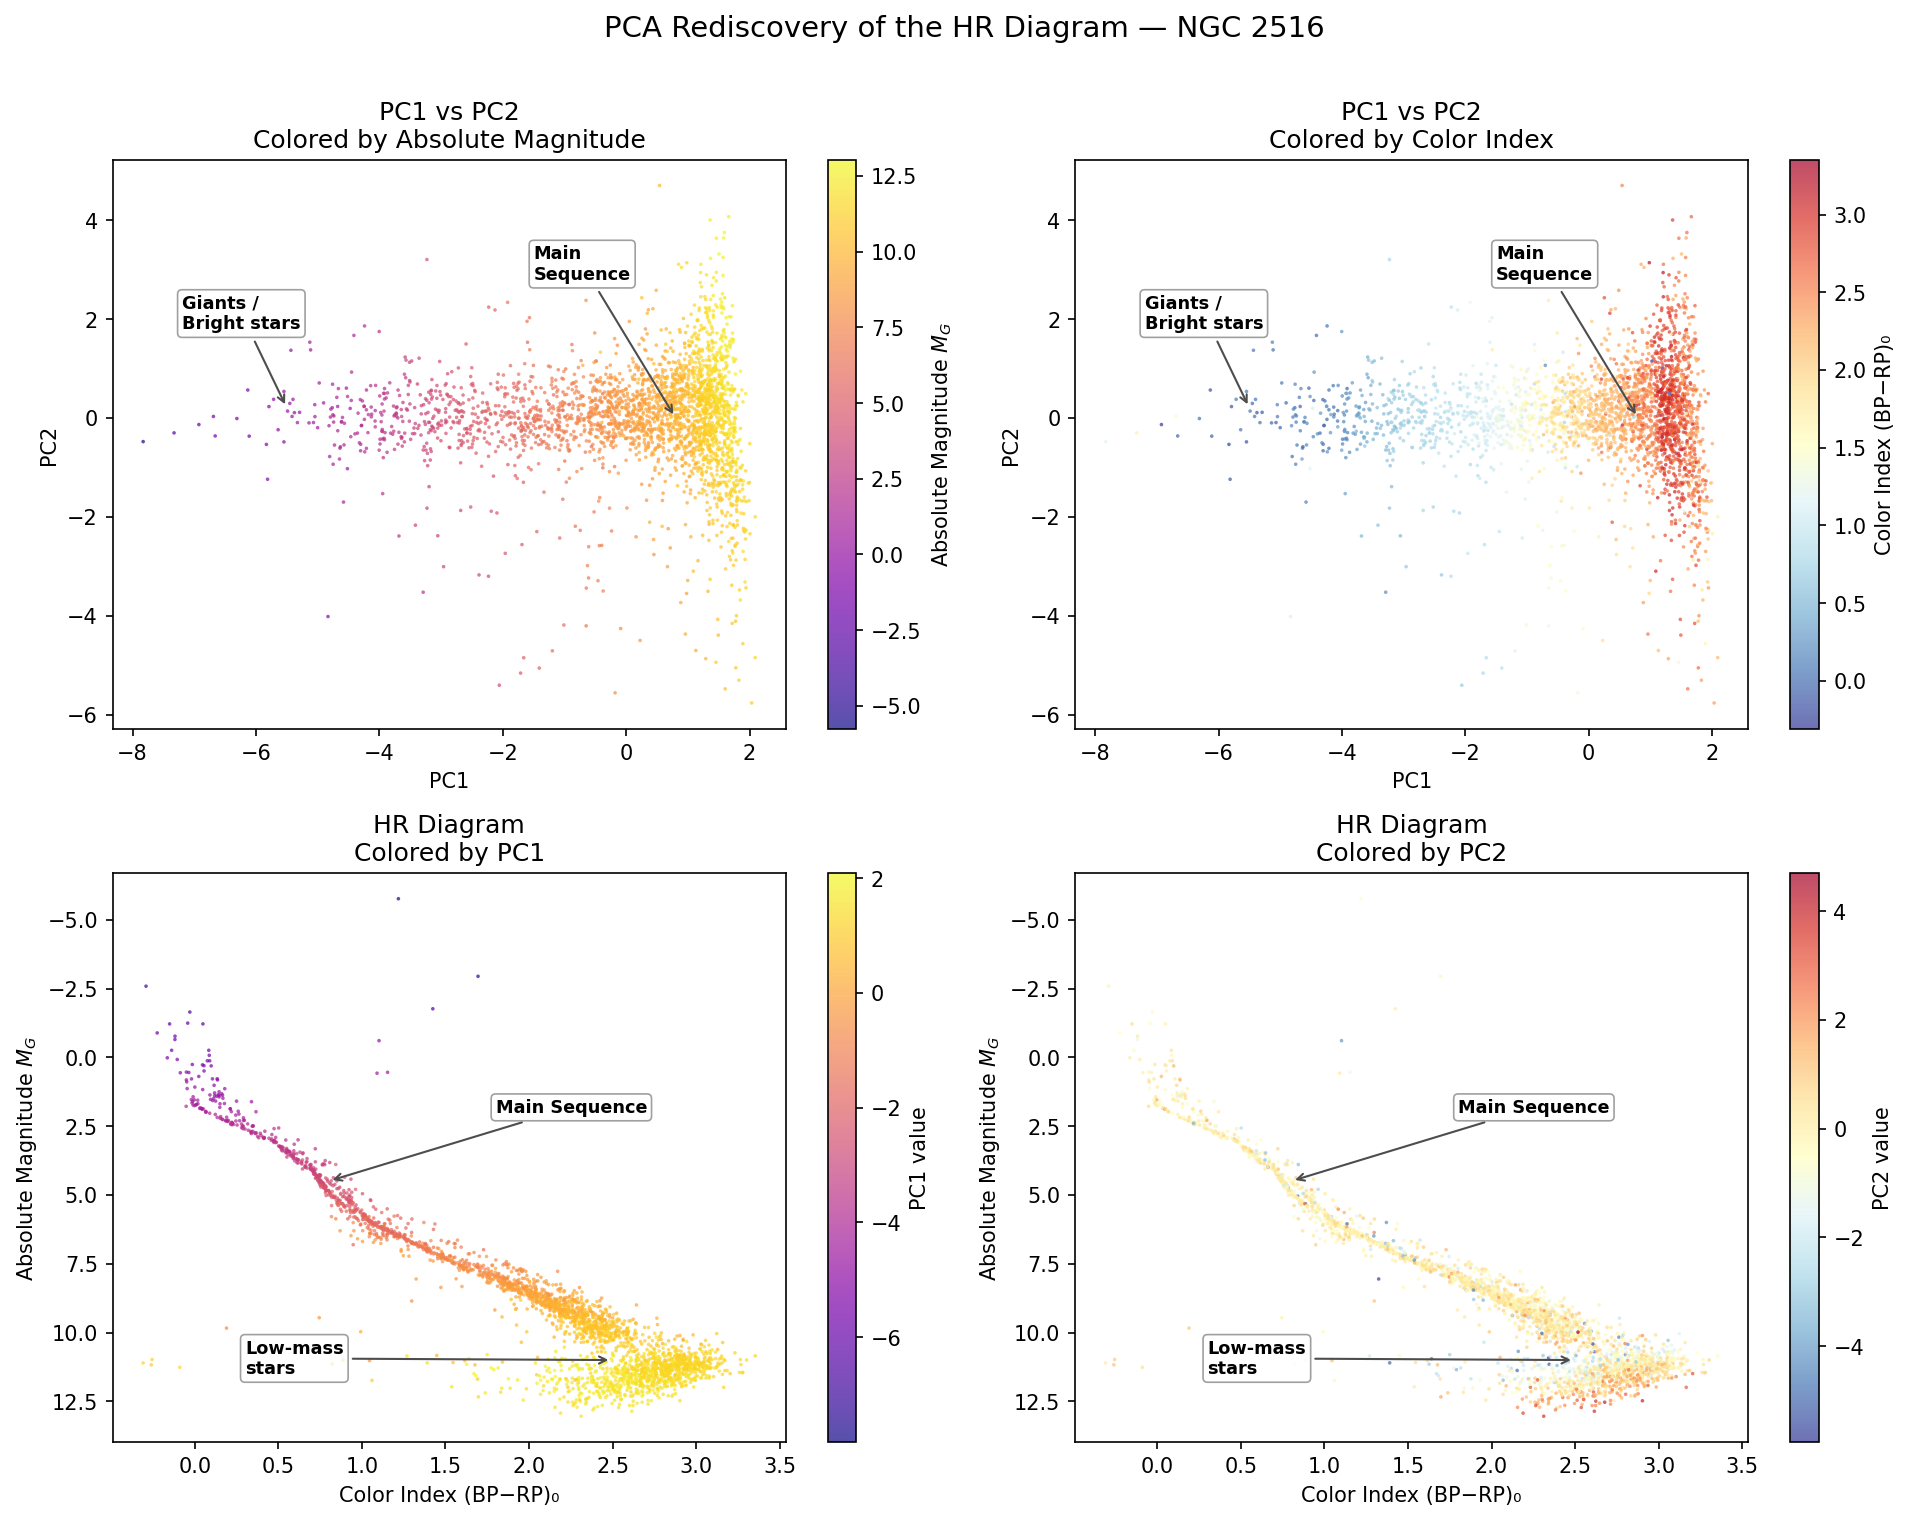
\includegraphics[width=0.90\linewidth]{hr_diagram_pca.png}
    \caption{PCA rediscovery of the HR diagram for NGC 2516. Top panels show the PCA embedding colored by absolute magnitude and color index respectively. Bottom panels show the HR diagram colored by PC1 and PC2 values.}
    \label{fig:pca_hr}
\end{figure}
PCA compressed the four input features into two principal components that together preserved $99.7\%$ of the total variance, showing that almost no information was lost in the reduction.\\
\newline
PC1 was the major axis explaining most of the variance and represented a pure brightness gradient. This is confirmed directly in the bottom left panel, where we see that PC1 varies smoothly and continually along the entire length of the main sequence, from strongly negative values at the bright, hot, blue end of the main sequence turnoff, to strongly positive values in the faint, cool, low-mass star region at the bottom right. The annotated giant and bright star population visible in the top left corner of the PCA space also separates nicely along this axis, separating from the main sequence at negative PC1 values. The model recovered this structure entirely on its own.\\
\newline
PC2 explains the remaining variance and plays a different role. In the bottom right panel we see that PC2 is almost constant along the main sequence, with most stars clustered around zero and only a gentle spread towards the low-mass end. It doesn't appear to be related to the star type or temperature much.  Instead it seems to be picking up some residual scatter that is likely related to small changes in parallax and depth within the cluster. This is smearing the data a bit, but doesn't tell us anything new or meaningful about the physical structure.\\
\newline
Looking at all four panels together it is clear that PCA was able to recover the main axis of the HR diagram on its own based on raw unlabeled photometric data. The PCA space naturally reveals the main sequence, the giant population and the low-mass star region. It's not that the model was trained to have these features, but rather that these are the dominant modes of variation in the underlying data of stars.

\section{Conclusion}
The goal of this project was to assess whether an unsupervised machine learning model could reconstruct the structure of the Hertzsprung-Russell diagram from raw, unlabelled stellar measurements alone. PCA is applied on four photometric and astrometric features obtained from open cluster NGC 2516 Gaia DR3 catalog without feeding the model with any prior knowledge of the stellar physics.\\
\newline
The results show that PCA achieved this goal. Two main components that accounted for $99.7\%$ of the total variance were enough to recreate the basic structure of the HR diagram. PC1 followed the main sequence as a continuous brightness gradient and naturally separated the giant population from the low-mass star region. This was not because the model was directed toward a known answer; rather, it was due to the fundamental physics of stellar populations genuinely being the primary source of variation in the data.\\ \newline
The exploration of UMAP and HDBSCAN as complementary methods revealed an important methodological lesson.  When you chain a non-linear dimensionality reduction step with a density-based clustering algorithm, you get pipeline bias. This means that HDBSCAN's boundaries showed the shape of UMAP's layout instead of real structure in the data. This finding shows that more complicated pipelines don't always lead to better science, and that every step in a machine learning workflow needs to be checked for any artifacts it might add.\\
\newline
In a broader sense, this study shows that the physical laws that govern the evolution of stars are structured enough that even a simple linear method can find basic astronomical relationships from scratch if given the right raw data. That's a significant outcome on its own.

\newpage
\bibliographystyle{apalike}
\bibliography{reference}
\end{document}
